%%% Ne pas modifier jusqu'à la ligne 25
\documentclass[a4paper,12pt]{book}
\usepackage[utf8]{inputenc}
\usepackage[french]{babel}
%%\usepackage{CJK}
\usepackage{yhmath}
\usepackage[left=2cm,right=2cm,top=3cm,bottom=2cm, headheight=1.5cm,headsep=1.5cm]{geometry}
%%\usepackage{CJKutf8}
\usepackage{amsfonts}
\usepackage{amsmath,amsfonts,amssymb,dsfont}
\usepackage{graphicx}
\usepackage{enumitem}		%\enumerate-resume
\usepackage[colorlinks=true,unicode={true},hyperindex=false, linkcolor=blue, urlcolor=blue]{hyperref}
\newcommand{\myref}[1]{\ref{#1} page \pageref{#1}}

\addto\captionsfrench{\def\tablename{Tableau}}  %légendes des tableaux
\renewcommand\thesection{\Roman{section}~-~} 
\renewcommand\thesubsection{\Roman{section}.\Alph{subsection}~-~} 
\renewcommand\thesubsubsection{\Roman{section}.\Alph{subsection}.\arabic{subsubsection}~-~} 

\newcommand{\conclusion}[1]{\newline \centerline{\fbox{#1}}}

\setcounter{secnumdepth}{3}
\parindent=0pt

\usepackage{fancyhdr}
\pagestyle{fancy}

\lhead{SJTU-ParisTech} 
%%%%%%%%%%%%%%%%%%%%%%%%%%%%%%%%%%
\chead{DM2}
\rhead{Daniel 518261910024}

\begin{document}
\renewcommand{\labelitemi}{$\blacktriangleright$}
\renewcommand{\labelitemii}{$\bullet$}


\section{Variétés allotropiques du carbone}
On supoose que les graphites et diamants sont considéré comme phases condensées idéaux. 
\subsection{}
On a le carbone graphite est plus stable que le carbone
diamant car $\boxed{\mu^\circ_G<\mu^\circ_D}$ dans cette température.
\subsection{}
On a $\boxed{V^G_m=\frac{V^G}{n}=\frac{m}{n\rho_G}=\frac{M}{\rho_G}}$. 
A.N. $\boxed{V^G_m=\frac{12.0*10^{-3}}{2260}=5.31*10^{-6}m^3mol^{-1}}$.

De même, $\boxed{V^D_m=\frac{M}{\rho_D}}$. 
A.N. $\boxed{V^D_m=\frac{12.0*10^{-3}}{3513}=3.42*10^{-6}m^3mol^{-1}}$
\subsection{}
À température constante, on a $\frac{du^*}{dP}=V_m^*$ pour un corps pur. 
On a donc $\frac{du^*}{dP}=V_m^*$, en intégrant entre $P^\circ$ et $P$, on a 
$\mu^*(T,P)=\mu^\circ(T)+V_m^*(P-P^\circ)$, où $P^\circ=1$ bar.

Donc $\boxed{\mu^G(P)=\mu_G^\circ+V_m^G(P-P^\circ)}$, et 
$\boxed{\mu^D(P)=\mu_D^\circ+V_m^D(P-P^\circ)}$
\subsection{}
À $T=298K$, pour préparer du carbone diamant à partir du carbone graphite, il faut que 
$\mu^G(P)>\mu^D(P)$, c'est à dire $$\mu_G^\circ+V_m^G(P-P^\circ)>\mu_D^\circ+V_m^D(P-P^\circ)$$
Finalement, on a $\boxed{P>P^\circ+\frac{\mu_D^\circ-\mu_G^\circ}{V_m^G-V_m^D}}$. 

A.N. $P>10^5+\frac{2870}{5.31*10^{-6}-3.42*10^{-6}}=1.52*10^9 Pa$, soit \fbox{$1.52*10^4$ bar}.
\section{Grandeurs de mélange}
\begin{figure}[h]
    \begin{center}
    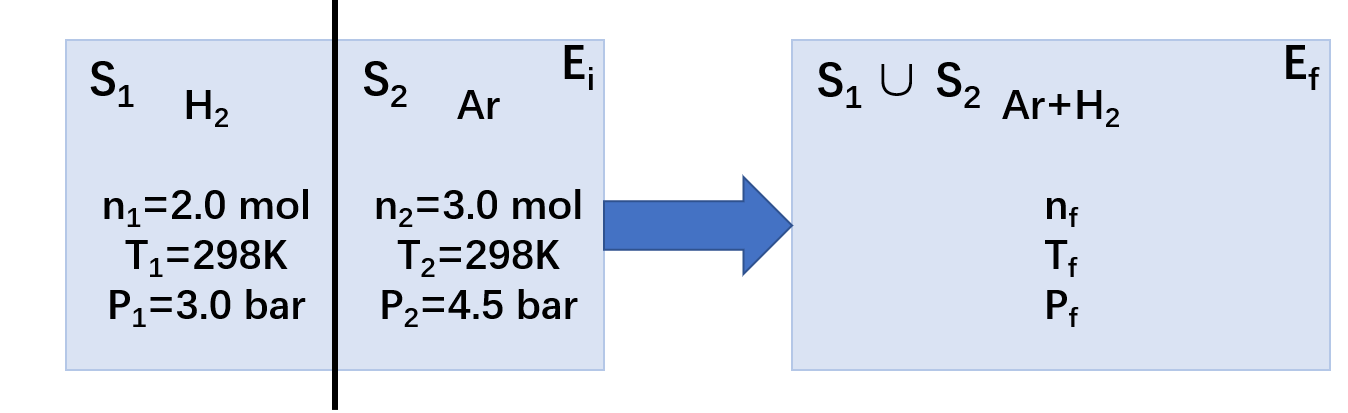
\includegraphics[scale=0.6]{dm2.png}
    \end{center}
    \caption{Figure du récipient adiabatique}
\end{figure}
\subsection{}
On applique le premier principe thermodynamique sur $S=S_1\cup S_2$: 
$$
\Delta U+\Delta E_c=W+Q
$$ 
On a $\Delta E_c=W=Q$ car c'est une transformation adiabatique, immobile macroscopiquement est isochore. 
Donc par additivité, on a $\Delta U=\Delta U_1+\Delta U_2=0$. Donc $$n_1C_{v,m,H_2}(T_f-T_1)+n_2C_{v,m,Ar}(T_f-T_2)=0$$
Finalemant, $\boxed{T_f=\frac{n_1T_1+n_2T_2}{n_1+n_2n_2}}$. A.N. $\boxed{T_f=\frac{2*298+3*298}{2+3}=298K}$
\subsection{}
C'est une transformation isotherme. Par additivité on a $n_f=n_1+n_2=5$mol.  
\begin{itemize}
    \item Par le théorème d'Euler, on a $\Delta_{mix}H=\Delta H_{m,1}n_1+\Delta H_{m,2}n_2$, où 
    $\Delta H_{m,i}=C_{p,m,i}\Delta T$, lorsque c'est une transformation isotherme, on a $dT=0$, d'où $\boxed{\Delta_{mix}H=0}$
    \item De même, on a $\Delta_{mix}S=\Delta S_{m,1}n_1+\Delta S_{m,2}n_2$, où 
    $\Delta S_{m,i}=C_{v,m,i}\ln\frac{T_f}{T_i}+R\ln\frac{V_f}{V_i}$, on a $dT=0$, donc $T_f=T_i$, et $V_f=2V_i$. 
    
    Alors, on a $\boxed{\Delta_{mix}S=n_fR\ln2}$. A.N. $\boxed{\Delta_{mix}S=5.0*8.314*0.69=29\,JK^{-1}}$
    \item Puisque $G=H-TS$, donc $dG=dH-TdS-SdT=dH-TdS$ lorsque $dT=0$. En intégrant entre $E_i$ et $E_f$, on a 
    $\boxed{\Delta_{mix}G=\Delta_{mix}H-T\Delta_{mix}S=-\ln{2}\,n_fRT}$. 
    
    A.N. $\boxed{\Delta_{mix}G=-0.69*5.0*8.314*298=-8.5*10^3J}$
\end{itemize}
Conclusion: cette transformation est irreversible comme $\Delta_{mix}S>0$, spontané comme $\Delta_{mix}G<0$, et l'enthalpie totale ne change pas. 
\end{document}